\documentclass[11pt]{article}

\usepackage[utf8x]{inputenc}
\usepackage{microtype}
\usepackage{geometry}

\usepackage{amsmath}
\usepackage{graphicx}
\usepackage{tikz}

\usepackage[font = {sf}, labelfont = {bf},
  labelsep = period, singlelinecheck = off]{caption}
\usepackage[font = {sf}]{floatrow}
\usepackage{tabularx}

\usepackage[numbers, round, sort&compress]{natbib}
\renewcommand{\citenumfont}{\itshape}  % Citations get italics numbers
\makeatletter
\renewcommand\NAT@open{(\hspace*{-0.3ex}}   % Tweak spacing.
\renewcommand\@biblabel[1]{#1.}  % Reference list doesn't use square brackets.
\makeatother

\usepackage[noblocks]{authblk}
\renewcommand{\Authsep}{, }
\renewcommand{\Authand}{ \& }
\renewcommand{\Authands}{ \& }
\renewcommand{\Affilfont}{\small}

% Load hyperref after the other stuff above.
\usepackage[pdfborder={0 0 0}]{hyperref}
\usepackage{hypernat}

\newcommand{\comment}[1]{\textbf{[#1]}}
\newcommand{\md}{\mathrm{d}}
\newcommand{\mT}{\mathrm{T}}
\renewcommand{\vec}[1]{\mathbf{#1}}
\newcommand{\mat}[1]{\mathbf{#1}}
\newcommand{\me}{\mathrm{e}}
\DeclareMathOperator{\Uniform}{Uniform}
\DeclareMathOperator{\Triangular}{Triangular}
\DeclareMathOperator{\Lognormal}{Lognormal}
\DeclareMathOperator{\BetaPERT}{Beta-PERT}

\newcommand{\labelPrefix}{S}
\renewcommand{\thesection}{\labelPrefix\arabic{section}}
\renewcommand{\theequation}{\labelPrefix\arabic{equation}}
\renewcommand{\thefigure}{\labelPrefix\arabic{figure}}
\renewcommand{\thetable}{\labelPrefix\arabic{table}}
\renewcommand{\figurename}{Fig.}
\renewcommand{\sectionautorefname}{Section}


\title{Supporting online material for\\
  \emph{Effectiveness of UNAIDS targets and HIV vaccination across 127
    countries}}

\author[1*]{Jan Medlock}
\author[2]{Abhishek Pandey}
\author[2]{Alyssa S.~Parpia}
\author[2]{Amber Tang}
\author[2]{Laura A.~Skrip}
\author[2]{Alison P.~Galvani}
\affil[1]{Department of Biomedical Sciences, Oregon State University,
  106 Dryden Hall, Corvallis, OR, 97331-4801, USA}
\affil[2]{Center for Infectious Disease Modeling and Analysis, Yale
  School of Public Health, 135 College Street, New Haven, USA}
\affil[*]{To whom correspondence should be addressed.  E-mail:
  \href{mailto:jan.medlock@oregonstate.edu}{
    \texttt{jan.medlock@oregonstate.edu}}}


\begin{document}

\maketitle

\section{Mathematical model}

We developed a continuous-time, compartmental model consisting of 8
health states (\autoref{model_diag}): susceptible to HIV infection
($S$), vaccinated against HIV ($R$), acute HIV infection ($A$),
undiagnosed HIV infection ($U$), diagnosed but untreated HIV infection
($D$), treated without viral suppression ($T$), viral suppression
($V$), and having AIDS ($W$).  Transitions between states are governed
by a series of differential equations parametrized using rates
estimated from other studies and from incidence and prevalence data
(Table \ref{model_param}).  The model is deterministic, but
uncertainty in the parameters is treated by running the model with
many different samples from the parameter distributions.

\begin{figure}
  \centering
  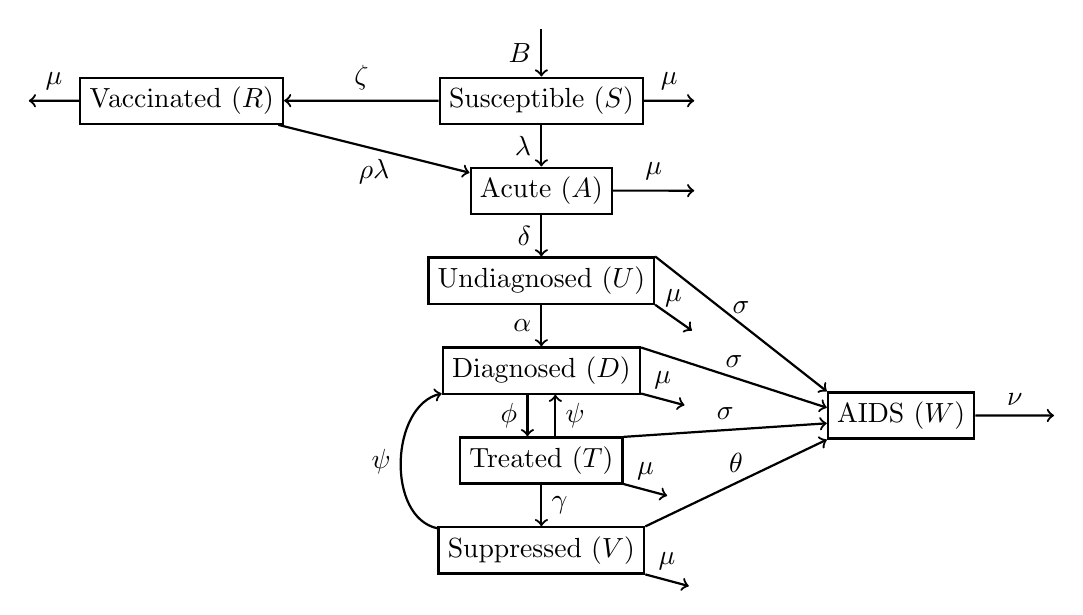
\begin{tikzpicture}[
  thick,
  scale = 1.142,
  compartment/.style = {draw},
  ]

  \node at (0, 5)
  [compartment, name = Susceptible] {Susceptible ($S$)};

  \node at (-4, 5)
  [compartment, name = Vaccinated] {Vaccinated ($R$)};

  \node at (0, 4)
  [compartment, name = Acute] {Acute ($A$)};

  \node at (0, 3)
  [compartment, name = Undiagnosed] {Undiagnosed ($U$)};

  \node at (0, 2)
  [compartment, name = Diagnosed] {Diagnosed ($D$)};

  \node at (0, 1)
  [compartment, name = Treated] {Treated ($T$)};

  \node at (0, 0)
  [compartment, name = Suppressed] {Suppressed ($V$)};

  \node at (4, 1.5)
  [compartment, name = AIDS] {AIDS ($W$)};

  \draw [->] (Susceptible) to node [left] {$\lambda$} (Acute);

  \draw [->] (Susceptible) to node [above] {$\zeta$} (Vaccinated);

  \draw [->] (Vaccinated) to node [below] {$\rho \lambda$} (Acute);

  \draw [->] (Acute) to node [left] {$\delta$} (Undiagnosed);

  \draw [->] (Undiagnosed) to node [left] {$\alpha$} (Diagnosed);

  \draw [->] (Diagnosed.240) to node [left] {$\phi$} (Treated.120);

  \draw [->] (Treated.60) to node [right] {$\psi$} (Diagnosed.300);

  \draw [->] (Treated) to node [right] {$\gamma$} (Suppressed);

  \draw [->] (Suppressed) to [out = 168, in = 193] node [left] {$\psi$} (Diagnosed);

  \draw [->] (Undiagnosed.12) to node [above] {$\sigma$} (AIDS.162);

  \draw [->] (Diagnosed.13) to node [above] {$\sigma$} (AIDS.174);

  \draw [->] (Treated.16) to node [above] {$\sigma$} (AIDS.186);

  \draw [->] (Suppressed.13) to node [above] {$\theta$} (AIDS.198);

  \draw [<-] (Susceptible) to node [left] {$B$} +(90: 0.8);

  \draw [->] (Susceptible) to node [above] {$\mu$} +(0: 1.7);

  \draw [->] (Vaccinated) to node [above] {$\mu$} +(0: -1.7);

  \draw [->] (Acute) to node [above] {$\mu$} +(0: 1.7);

  \draw [->] (Undiagnosed.348) to node [above] {$\mu$} +(325: 0.5);

  \draw [->] (Diagnosed.347) to node [above] {$\mu$} +(345: 0.5);

  \draw [->] (Treated.344) to node [above] {$\mu$} +(345: 0.5);

  \draw [->] (Suppressed.347) to node [above] {$\mu$} +(345: 0.5);

  \draw [->] (AIDS) to node [above] {$\nu$} +(0: 1.7);

\end{tikzpicture}


%%% Local Variables:
%%% mode: latex
%%% TeX-master: "model"
%%% End:

  \caption{Model diagram.}
  \label{model_diag}
\end{figure}

\begin{table}
  \begin{center}
    \begin{tabularx}{\textwidth}{lXlll}
      \hline
      & Definition & Value & Reference \\
      \hline
      $\delta$	& Rate of leaving acute infection
      & $\Triangular$(2, 4.14, 9.6)\;y$^{-1}$
      & \cite{Hollingsworth2008-iy} \\
      $\sigma$	& Rate of developing AIDS without viral suppression
      & 0.1064\;y$^{-1}$ & \cite{Morgan2002-cq} \\
      $\theta$ & Rate of developing AIDS with viral suppression
      & See eq.~(\ref{theta}) & --- \\
      $\gamma$ & Rate of viral suppression
      & $\Uniform$(0.5, 1.5)\;y$^{-1}$
      & \cite{Currie2009-yz} \\
      $\nu$ & Death rate from AIDS & 0.5\;y$^{-1}$
      & \cite{Morgan2002-cq} \\
      $\rho$ & Vaccine efficacy & 50\%\,[30\%, 70\%] & --- \\
      $\omega$	& Reduction in lifetime with viral suppression
      & $\Uniform$(5, 8)\;y
      & \cite{Unaids2014-ue, Samji2013-kf} \\
      $\tau_{A}$ & Transmissibility during acute phase
      & $\Triangular$(0.0039, 0.0082, 0.0150)
      & \cite{Skarbinski2015-ni,Wawer2005-us}\\
      $\tau_{U}$ & Transmissibility after acute phase
      & $\Triangular$(0.00077, 0.0014, 0.00251)
      & \cite{Hughes2012-so} \\
      $\varepsilon$ & Relative transmissibility with
      viral suppression & $\BetaPERT$(0.08, 0.002, 0.57)
      & \cite{Donnell2010-xo} \\
      $n$ & Sex acts per year & $\Uniform$(96, 108)
      & \cite{Wawer2005-us,Abdool_Karim2010-cm}\\
      $\mu$ & Background death rate & Country specific
      & \cite{World_Development_Indicators2013-ee} \\
      $B$ & Birth rate & Country specific
      & \cite{World_Development_Indicators2013-ee, WorldBankpg} \\
      $\alpha$ & Diagnosis rate & See eqs.~(\ref{target_rates}) & --- \\
      $\phi$ & Treatment rate & See eqs.~(\ref{target_rates}) & --- \\
      $\psi$ & Rate of relapse to untreated & See eqs.~(\ref{target_rates})
      & --- \\
      $\zeta$ & Vaccination rate & See eqs.~(\ref{target_rates}) & --- \\
      \hline
    \end{tabularx}
    \caption{Model parameters. $\Triangular$, $\Uniform$,
      and $\BetaPERT$ are sampling distributions: see text for a
      full description.  For vaccine efficacy, $50\%$ was the
      baseline, and $30\%$ and $70\%$ were also used in scenario
      analysis.}
    \label{model_param}
  \end{center}
\end{table}


Birth and death.

People living with HIV (PLHIV) are divided among the acutely infected,
undiagnosed, diagnosed, treated, viral suppression and AIDS
compartments. People susceptible to HIV ($S$) progress to the
acute-infection phase ($A$) according to the force of infection
($\lambda$), which depends on the HIV transmission rate, estimated
from the country-specific incidence and prevalence data
(\autoref{model_fitting}), adjusted for the current number of acutely
infected, untreated or ineffectively treated, and viral suppression
PLHIV.  Acute infection is characterized by high viral loads and lasts
an average of 2.90 [95\% confidence interval 1.23, 6.00]\;months
\cite{Hollingsworth2008-iy}.  (We converted these durations to rates
like $1 / 2.90\;\text{month$^{-1}$} \approx 4.14\;\text{y$^{-1}$}$ and
set the parameter using random samples from
$\Triangular(2, 4.14, 9.6)\;\text{y$^{-1}$}$ to capture the
uncertainty in its value.)  We assumed that people remain undiagnosed
during their acute infection phase and during at least some of the
subsequent period of clinical latency (i.e., the undiagnosed
compartment $U$). After acute infection, people move into the chronic
undiagnosed class ($U$).  People in the undiagnosed class will be
diagnosed at the rate $\alpha$, which is determined by the country's
current diagnosis level and its diagnosis target.  Diagnosed people
($D$) transition to the treated compartment ($T$) upon starting ART at
the rate $\phi$, dependent on the country's current treatment level
and its treatment target.  After some time, treated people then to the
viral-suppression class ($V$), at the rate $\gamma$.  We took $\gamma$
as a random sample from $\Uniform(0.5, 1.5)\;\text{y$^{-1}$}$, that
is, viral suppression occurs after between 8 months and 2 years on
treatment \cite{Currie2009-yz}.  The disengagement from treatment
moves people from treated ($T$) and viral suppression ($V$) at the
rate $\psi$, dependent on the current level of viral suppression and
the country's target, back to the diagnosed class ($D$).

PLHIV without viral suppression (compartments $U$, $D$, and $T$)
develop AIDS (compartment $W$) after an average duration of 10.4 y
\cite{Morgan2002-cq}, giving the transition rate
$\sigma = 0.1064\;\text{y$^{-1}$}$.  People who have achieved viral
suppression ($V$) develop AIDS at rate $\theta$, slower than PLHIV
without viral suppression.  People with viral suppression are
estimated to live 5--8 y shorter lives than the non-HIV infected
\cite{Unaids2014-ue, Samji2013-kf}, which we quantified by randomly
sampling the parameter $\omega$ from $\Uniform(5, 8)\;\text{y}$.
Assuming no relapse to untreated, the duration of viral suppression is
\begin{equation}
  \frac{1}{\theta + \mu} = \frac{1}{\mu} - \omega - \frac{1}{\nu}.
\end{equation}
The term to the left of the equals sign is the time until leaving
viral suppression by either progression to AIDS (at rate $\theta$) or
background mortality (at rate $\mu$).  The term to the right of the
equals sign is the lifespan of the non-HIV infected, minus the
reduction in life due to having HIV with viral suppression, minus the
duration of the AIDS stage.  Solving for $\theta$ gives the rate of
progression to AIDS with viral suppression as
\begin{equation}
  \label{theta}
  \theta = \frac{1}{1/\mu - \omega - 1/\nu} - \mu.
\end{equation}

Susceptible people are vaccinated at rate $\zeta$, transitioning into
the vaccinated compartment ($R$), where the vaccine reduces their
force of infection by the efficacy factor $\rho$.

Transition rates between the undiagnosed ($U$), diagnosed ($D$),
treated ($T$), and viral-suppression classes ($V$) are determined by
the proportion of PLHIV diagnosed
\begin{equation}
  p_D = \frac{D + T + V + W}{A + U + D + T + V + W},
\end{equation}
the proportion of diagnosed people on ART
\begin{equation}
  p_T = \frac{T + V + W}{D + T + V + W},
\end{equation}
the proportion of people on ART who have
achieved viral suppression
\begin{equation}
  p_V = \frac{V}{T + V},
\end{equation}
and the proportion of susceptible people vaccinated is
\begin{equation}
  p_R = \frac{R}{S + R}.
\end{equation}

We can implement the vaccination compartment in the same way as the
other controls. When we begin vaccination in 2020 (also 2025 in
scenario analysis), the initial vaccination level is 0\%. The coverage
will increase linearly by 25\% per year (also 10\% per year in
scenario analysis). The coverage will continue to increase linearly
until it reaches 70\% coverage (50\% \& 90\% in scenario analysis) and
then stay constant for the remainder of the time period.

95--95--95 goal is implemented subsequently after meeting 90--90--90
by 2020 by increasing $p_D$, $p_T$, and $p_V$ to 95--95--95 levels by
2030 linearly. \comment{@Jan, We use the Heaveside function here too?
JM: Yes.  I'll write it at some point.}

The rates are applied when the proportions of $p_D$, $p_T$, $p_V$, and
$p_R$ are below the target levels:
\begin{equation}
  \label{target_rates}
  \begin{split}
    \alpha(t) &= \alpha_{\max} H\left(p_D^*(t) - p_D(t)\right),
    \\
    \phi(t) &= \phi_{\max} H\left(p_T^*(t) - p_T(t)\right),
    \\
    \psi(t) &= \psi_{\max} H\left(p_V(t) - p_V^*(t)\right),
    \\
    \zeta(t) &= \zeta_{\max} H\left(p^{*}_{R}(t) - p_{W}(t)\right),
  \end{split}
\end{equation}
where $H(x)$ is the Heaviside function
\begin{equation}
  H(x) =
  \begin{cases}
    0 & \text{if $x < 0$},
    \\
    1 & \text{if $x > 0$}.
  \end{cases}
\end{equation}

The discontinuity of the Heaviside function makes numerical solution
difficult.  Instead, replace $H$ with the continuous piecewise linear
function
\begin{equation}
  H(x) =
  \begin{cases}
    0 & \text{if $x < 0$},
    \\
    x / \chi & \text{if $0 \leq x \leq \chi$},
    \\
    1 & \text{if $x > \chi$},
  \end{cases}
\end{equation}
with some small value of $\chi$.

The model equations are
\begin{equation}
  \label{model_eqns}
  \begin{split}
    \frac{\md S}{\md t} &= B N - \lambda S - \zeta S- \mu S,
    \\
    \frac{\md R}{\md t} & = \zeta S - (1 - \rho) \lambda R - \mu R,
    \\
    \frac{\md A}{\md t} &= \lambda S + (1 - \rho) \lambda R - \delta A - \mu A,
    \\
    \frac{\md U}{\md t} &= \delta A - \alpha U - \mu U - \sigma U,
    \\
    \frac{\md D}{\md t} &=  \alpha U + \psi T + \psi V
    - \phi D - \mu D - \sigma D,
    \\
    \frac{\md T}{\md t} &= \phi D - \psi T - \gamma T - \mu T
    - \sigma T,
    \\
    \frac{\md V}{\md t} &= \gamma T - \psi V - \mu V - \theta V,
    \\
    \frac{\md W}{\md t} &= \sigma U + \sigma D + \sigma T + \theta V -
    \nu W,
  \end{split}
\end{equation}
with force of infection
\begin{equation}
  \label{force_of_infection}
  \begin{split}
    \lambda &= \frac{\beta_A A + \beta_U (U + D + T) + \beta_T V}{N},
    \\
    N &= S + R +  A + U + D + T + V,
    \\
    \beta_x &= T \left[1 - (1 - \tau_x)^n\right]
    \text{ for $x \in \{A, U, T\}$},
    \\
    \tau_T &= \varepsilon \tau_U.
  \end{split}
\end{equation}

The targets for the proportions $p_D$, $p_T$, and $p_V$ in the
achievement of 90--90--90 all operate under the following assumption:
if the initial level $p_x(0)$ is less than $90\%$, the proportion will
increase linearly in the first 5 years and then stay at $90\%$ for the
remaining time; and if the initial level is at $90\%$ or above, the
proportion will remain constant for the duration of the study:
\begin{equation}
  p_x^*(t)
  = p_x(0) + \left[
    \max\left\{0.9, p_x(0)\right\} - p_x(0)
  \right]
  \min\left\{\frac{t}{5}, 1\right\},
\end{equation}
for $x \in \{D, T, V\}$.


$\Uniform(a, b)$ is the uniform random variable with minimum $a$
and maximum $b$: it has density function
\begin{equation}
  \label{uniform}
  p_{\Uniform}(x) =
  \begin{cases}
    \frac{1}{b - a} & \text{if $a \leq x \leq b$,}
    \\
    0 & \text{otherwise.}
  \end{cases}
\end{equation}
We defined the mode for the uniform distribution to be the midpoint
$\frac{b - a}{2}$.
%
$\Triangular(a, b, c)$ is the triangular random variable
distribution with minimum $a$, mode $b$, and maximum $c$: it has
density function
\begin{equation}
  \label{triangular}
  p_{\Triangular}(x) =
  \begin{cases}
    \frac{2 (x - a)}{(c - a)(b - a)} & \text{if $a \leq x \leq b$,}
    \\
    \frac{2 (c - x)}{(c - a)(c - b)} & \text{if $b \leq x \leq c$,}
    \\
    0 & \text{otherwise.}
  \end{cases}
\end{equation}
$\BetaPERT(a, b, c)$ is the beta-PERT probability distribution
\cite{malcom1959} with minimum $a$, mode $b$, and maximum $c$: it has
density function
\begin{equation}
  \label{betaPERT}
  p_{\BetaPERT}(x) =
  \begin{cases}
    \frac{(x - a)^{v - 1} (c - x)^{w - 1}}{(c - a)^{v + w - 2} B(v, w)}
    & \text{if $a \leq x \leq c$,}
    \\
    0 & \text{otherwise,}
  \end{cases}
\end{equation}
where
\begin{equation}
  \begin{split}
    \mu &= \frac{a + \lambda b + c}{\lambda + 2},
    \\
    v &= \frac{(\mu - a)(2 b - a - c)}{(b - \mu) (c - a)},
    \\
    w &= \frac{v (a - \mu)}{\mu - c},
  \end{split}
\end{equation}
and $B(v, w)$ is the standard beta function \cite[\S 6.2]{davis1972}.
We used the standard value of $\lambda = 4$.
%
$\Lognormal(\mu, \sigma^2)$ is the lognormal random variable: it has
density function
\begin{equation}
  p_{\Lognormal}(x) = \frac{1}{x \sigma \sqrt{2 \pi}}
  \exp\left(- \frac{\left(\log x - \mu\right)^2}{2 \sigma^2}\right).
\end{equation}



Projections were generated for each country through model simulations
using 1000 random samples from published parameter distributions
(table S1, Supplementary text) and the country-specific estimated
distribution of the transmission rate. We evaluated the global and
country-level impacts of meeting the UNAIDS targets and vaccine
deployment on four outcome measures: HIV incidence, PLHIV, PLAIDS, and
AIDS-related deaths between 2015 and 2035. Our base-case scenario
assumed maintenance of the status quo: that 2015 levels of the
proportion of PLHIV diagnosed (pD), proportion of those diagnosed on
ART (pT), and proportion of those on treatment who have achieved viral
suppression (pV) continue unchanged until 2035. The intervention
scenarios were (1.) the attainment of the 90–90–90 target by linear
increases in pD, pT, and pV until 2020 followed by maintenance of
those levels until 2035, and (2.) linear increase in the diagnosis and
treatment levels to the 90–90–90 target by 2020, a linear increase
from 90–90–90 to the 95–95–95 target by 2030, and maintenance of the
95–95–95 levels to 2035. (For 90–90–90, if any initial level was above
90\%, it was kept constant going forward so that the intervention did
not worsen coverage.  Likewise, for 95–95–95, any initial level above
95\% was kept constant.)  For vaccination, we assumed deployment of a
vaccine with 50\% efficacy in 2020 with coverage increasing linearly
by 25\% per year, continuing up to 70\% at 2.8 years post-rollout, and
maintaining constant 70\% coverage thereafter.  We also performed a
partial rank correlation coefficient (PRCC) sensitivity analysis for
each model parameter and a scenario analysis to account for
uncertainty in the profile of the prospective vaccine.



\section{Source code}

The source code for the model and analysis tools is publicly available
at \url{https://github.com/janmedlock/HIV-95-vaccine/}
\cite{medlock2016-git}.


\section{Data sources}
\label{data_sources}

For 127 countries, we found sufficient data to parametrize our model:
these data consisted of estimates of longitudinal HIV incidence and
prevalence for ages 15–49 years starting as early as 1990 in some
countries and running through 2015, along with basic demographics
(\autoref{data_sources}).

Several sources provided information to parameterize our model at the
country level. Demographic data, including population growth rate
\cite{WorldBankpg}, death rate
\cite{World_Development_Indicators2013-ee}, and number of people aged
15--49 years \cite{The_World_Bank2016-fd} were obtained from the World
Bank. Longitudinal HIV incidence and prevalence estimates for the
15--49 age group, spanning from as early as 1990 to 2015, was
primarily derived from the AIDSinfo database produced by UNAIDS
\cite{Unaids2016-an}. Other sources included UNAIDS Country Progress
Reports \cite{Unaids2016-am} published from 2012 to 2016 and AIDS Data
Hub \cite{AIDSdatahub-fg}, which compiles data from UNAIDS, UNICEF,
WHO, and the Asian Development Bank. These sources were also used to
inform the initial conditions for the model: the number of people who
have been diagnosed with HIV, who are on ART, and who have viral
suppression or have been retained on treatment for at least 12
months. Where data were not available from these sources, alternative
resources such as peer-reviewed journal articles and country health
ministry reports were consulted.  We found sufficient data to
parametrize our mathematical modeling for 127 countries.  See
Supplemental data files for full information on data sources for each
country.  The data files are also available in the public source-code
repository \cite{medlock2016-git}.


\section{Model fitting}
\label{model_fitting}

Using available historical data for incidence and prevalence, and
published transmission estimates, we estimated transmission rates for
people with acute infection, unsuppressed viral load and suppressed
viral load. Our calibration method provided a recent snapshot of
country-specific transmission, while using historical data to smooth
out variations.

We first estimated country-specific rates of HIV transmission for each
of the available historical data point for incidence and
prevalence. The calculation involved a simplified force of infection
that initially assumed no differences in transmission risk among
acute, unsuppressed, suppressed, and AIDS classes due to the general
lack of historical data on diagnosis and treatment. We calculated a
time-independent aggregate transmission rate by taking an exponential
weighted mean of the historical (i.e., time-dependent) transmission
rates for each given country (\autoref{transmission_rate}). The
aggregate transmission rate was then combined with estimated HIV
transmission risk by stage of HIV infection
\cite{Hollingsworth2008-iy} and treatment status \cite{Wawer2005-us}
to calculate separate transmission rates for unsuppressed, acute, and
viral-suppression people. These rates were used to simulate model
projections through 2035.



{We calibrated longitudinal HIV incidence and prevalence data from
  1990 to 2015 incidence in addition to data on $p_{D}$, $p_{T}$ and
  $p_{V}$ levels in 2015 to estimate the rate of transmission for each
  country. The calculation involved a simplified force of infection:}

\begin{align}
  \label{foi}
  \begin{split}
  \lambda(t) &  =    \frac{\beta_{A} A + \beta_{U}(U+D+T)+\beta_{V}V+0
               W}{N} \\
             &  =  \beta \frac{I}{N},
             \end{split}
\end{align}
where $\beta$ is the estimated time-independent aggregate transmission rate under the
assumption that there is no difference in transmission risk among acute, unsuppressed, suppressed, and AIDS classes.

$I = A+U+D+T+V+W$ is the total number of people living with HIV. Therefore, the per-capita
incidence is
\begin{equation}
i(t) = \lambda(t) \frac{S(t)}{N(t)}
= \beta(t) \frac{I(t)}{N(t)} \frac{S(t)}{N(t)} =\beta(t) p(t) (1-p(t)),
\end{equation}
where $p(t)$ is the prevalence. Thus, we can estimate the
transmission rate at each historical time point using the incidence
and prevalence data,
\begin{equation}
  \label{trans_rate}
  \beta(t) = \frac{i(t)}{p(t)(1-p(t))}
\end{equation}


We estimated the time-independent aggregated transmission rate ($\beta$)
by taking the exponential weighted mean of transmission rates
(\ref{trans_rate}).


Rearranging equation (\ref{foi}), the transmission rate for PLHIV
without viral suppression can be written as
\begin{equation}
\label{betaU}
  \beta_{U} = \frac{\beta I}{\frac{\beta_{A}}{\beta_{U}}A +
    U+D+T+\frac{\beta_{V}}{\beta_{U}}V}
\end{equation}


Next, we assumed that the relative risk of acute HIV transmission
($\beta_{AU} = \beta_{A}/\beta_{U}$) and virally suppressed HIV
transmission ($\beta_{VU} = \beta_{V}/\beta_{U}$) with respect to the
unsuppressed transmission remains constant worldwide and calculated
these values using the data from Rakai, Uganda \cite{Wawer2005-us}. The aggregate
rate of transmission ($\beta$) can then be combined with equations \ref{betaU} to calculate transmission
rates for unsuppressed PLHIV, acute PLHIV and suppressed PLHIV as,
\begin{align}
  \beta_{U} & = \frac{\beta I}{\beta_{AU}A +
              U+D+T+\beta_{VU}V}, \\
  \beta_{A} & = \beta_{AU}\beta, \\
  \beta_{V} & = \beta_{VU} \beta.
\end{align}
that we use to simulate our model forward and project results up to 2035.
\\

\comment{Need to add stuff about how we generate distribution of
  transmission rates}




\begin{figure}
  \centering
  \includegraphics{../Codes/plots/transmission_rate.pdf}
  \caption{Country-specific transmission rates were calculated based
    on the relative contributions of people with acute infection,
    unsuppressed viral load or suppressed viral load to overall
    transmission (\autoref{model_fitting}). The estimates were
    calibrated to data on country-level incidence and/or prevalence to
    account for variation in historical incidence while accurately
    reflecting recent HIV rates.}
  \label{transmission_rate}
\end{figure}


\section{Analysis}

We evaluated the global and country-specific impacts of meeting the
UNAIDS targets and vaccine deployment on four outcome measures: HIV
incidence, PLHIV, number of people with AIDS, and AIDS-related deaths
between 2015 and 2035. Calibrating our model to historical data on
prevalence and incidence, we projected the anticipated trajectories of
the outcomes using country-specific transmission rates across the
intervention scenarios outlined below.  Our base-case scenario assumed
maintenance of the status quo: that 2015 levels of the proportion of
PLHIV diagnosed ($p_{D}$), proportion of those diagnosed on ART
($p_{T}$), and proportion of those on treatment who have achieved
viral suppression ($p_{V}$) continue unchanged until 2035.  The
intervention scenarios were 1.) the attainment of the 90--90--90
target by linear increases in $p_{D}$, $p_{T}$, and $p_{V}$ until 2020
followed by maintenance of those levels until 2035, and 2.) linear
increase in the diagnosis and treatment levels to the 90--90--90
targets by 2020, a linear increase from 90--90--90 to the 95--95--95
target by 2030, and maintenance of the 95--95--95 levels to 2035. (For
90--90--90, if any initial level was above 90\%, it was kept constant
going forward so that the intervention did not worsen coverage.
Likewise, for 95--95--95, any initial level above 95\% was kept
constant.)  For vaccination, we assumed deployment of a vaccine with
50\% efficacy in 2020 with coverage increasing linearly from 0\% to
50\% at 2 years post-rollout and maintaining constant coverage after
reaching 70\%. The added benefit of vaccination was considered in the
context of status quo diagnosis and treatment, achieving the UNAIDS
90–90–90 goal by 2020 followed by maintenance, and achieving the
95–95–95 goal by 2030 followed by maintenance.  Projections were
generated through model simulations based on published parameter
distributions (\autoref{model_param}) and country-specific estimated
transmission rate distributions. The parameters were sampled using
latin hypercube sampling \cite{blower1994} and the variance reduction
technique of running different interventions with random parameter
values \cite{shechter2006}.

Model outcomes were projected until 2035 for each of the 127 countries
with sufficient data on status quo rates of diagnosis and treatment
and on historical incidence or prevalence
(\hyperref[effectiveness_Global]{\autoref*{effectiveness_Global}}--\ref{effectiveness_Zimbabwe}). The
median estimates with interquartile ranges are presented between 2015
and 2035 for number of PLHIV, per-capita incidence, PLAIDS, and number
of HIV-related deaths under the status quo and five intervention
scenarios: vaccination only, attaining the UNAIDS 90--90--90 target,
attaining the 90--90--90 target and vaccination, attaining the UNAIDS
95--95--95 target, and attaining the 95--95--95 target and
vaccination.  The results from the country were aggregated to the
regional and global levels by adding the numbers of people in each
compartment over time and then PLHIV, per-capita incidence, PLAIDS,
and HIV-related deaths were calculated from the aggregates.

We calculated partial rank correlation coefficients (PRCC)
\cite{blower1994} to measure the independent effect of each parameter
on model projections of HIV incidence (\autoref{PRCCs}). Furthermore,
due to uncertainty surrounding the prospective vaccine, we obtained
model projections using six additional vaccine scenarios by
considering alternative estimates of efficacy (30\%, 70\%), coverage
(50\%, 90\%), speed of scale up (10\% coverage per year), and first
year of availability (2025).

\begin{figure}
  \centering
  \includegraphics{../Codes/plots/prcc.pdf}
  \caption{Parameter sensitivity of model global infections averted
    from 2015 to 2035.}
  \label{PRCCs}
\end{figure}


\clearpage
\bibliographystyle{science_nat}
\bibliography{supplementary_text}


\appendix
\newpage
\vspace*{3in}
\section{Model results by region and country}
\newpage
\input{../Codes/plots/effectiveness_all/all}


\end{document}
